\documentclass[border={0pt 0.7cm 0pt 0.7cm}]{standalone}
\usepackage{tikz}
\usepackage{ctex,siunitx,ninecolors}
\usepackage{tkz-euclide}
\usepackage{amsmath}
\usetikzlibrary{patterns, calc}
\usetikzlibrary {decorations.pathmorphing, decorations.pathreplacing, decorations.shapes,}
\begin{document}
\small
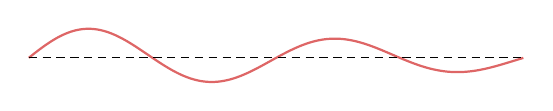
\begin{tikzpicture}[>=stealth, xscale=0.5, domain=0:4*pi, samples=2000]
  \draw [thick, domain=0:4*pi,red6]  plot (\x,{(1-0.05*\x)*0.4*sin(\x r)});
  \draw[densely dashed] (0,0)--(12.56,0);
\end{tikzpicture}
\end{document}